 \chapter{Estado del arte}\label{cap:estadoarte}

	El objetivo de este capítulo es dar una visión general de los sistemas o acciones de control que actualmente son utilizados en la industria para el control de magnitudes físicas, concretamente para controlar la temperatura. En este TFG el sistema de control es una pieza fundamental, ya que es el encargado de generar la señal de control que se aplica en todo momento al sistema de refrigeración para que la sala alcance la temperatura deseada.

	Primero se va a explicar el concepto de sistema de control y sus configuraciones más importantes. Después, se van a exponer las principales acciones de control usadas en la industria para realizar el control de la temperatura. Por último, se expone la situación actual en cuanto al control automático de la temperatura en los centros de datos.

\section{Sistema de control}

	Un sistema de control puede definirse como un conjunto de dispositivos encargados de administrar, dirigir o regular el comportamiento de otro sistema, y así obtener los resultados deseados. Si enfocamos la definición a este trabajo, la variable a controlar es la temperatura de la sala y esto se consigue controlando el comportamiento del sistema de refrigeración, es decir, su temperatura de funcionamiento o \textit{setpoint}. 

	Abstrayéndose de la aplicación concreta, un sistema de control sencillo básicamente posee una entrada de referencia y una salida o variable controlada. La entrada de referencia representa el valor que se desea que tenga la variable controlada y la función del sistema de control es conseguir que la variable controlada alcance ese valor. Dependiendo de si el sistema de control usa o no la entrada de referencia, podemos distiguir 2 tipos de configuración \cite{control1}:

	\textbf{Configuración en lazo abierto:} la variable controlada no es comparada con la entrada de referencia. Por lo tanto, cada valor de la entrada de referencia corresponde a una condición de operación fija. Esta configuración se usa principalmente en sistemas donde no hay perturbaciones y se conoce la relación entre la entrada y la salida. El motivo es que estos sistemas son fáciles de construir y mantener pero son más sensibles a las perturbaciones externas y la precisión de la salida depende de la calibración de los componentes, por lo que es complicado lograr que sean exactos. En la figura \ref{fig2_1:esquemacontrol} puede verse un esquema de esta configuración.

\begin{figure}[htbp]
	\centering
	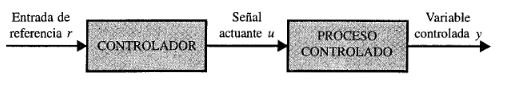
\includegraphics[width=120mm, height=20mm]{imagenes/capitulo2/2_1_1LazoAbierto}
   	\caption{Sistema de control en lazo abierto. Fuente: \textit{Benjamin C. Kuo}\cite{control2}}
   	\label{fig2_1:esquemacontrol}
\end{figure}

	\textbf{Configuración en lazo cerrado:} la variable controlada es medida y comparada con la entrada de referencia, generando una señal de error. Dicha señal es utilizada por el controlador para generar la señal de control y lograr que la variable controlada alcance el valor de la entrada. Los sistemas que usan esta configuración son más inmunes frente a las perturbaciones externas y más económicos en el sentido de que puede utilizar componentes más baratos y menos precisos para conseguir el ajuste deseado. Sin embargo, tienen mayores problemas de estabilidad porque el lazo de realimentación puede convertir un sistema estable en uno inestable. En la figura \ref{fig2_2:esquemacontrol} puede verse un esquema de esta configuración.

\begin{figure}[htbp]
	\centering
	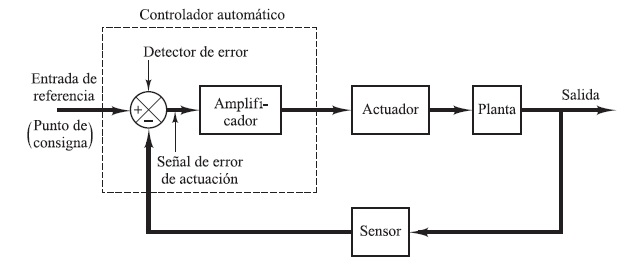
\includegraphics[width=110mm, height=40mm]{imagenes/capitulo2/2_1_2LazoCerrado}
   	\caption{Sistema de control en lazo cerrado. Fuente: \textit{Katsuhiko Ogata} \cite{control1}}
   	\label{fig2_2:esquemacontrol}
\end{figure}

	Hay que recalcar que los sistemas de control pueden tener múltiples entradas y múltiples salidas. Sin embargo, estas cuestiones no son tratadas en este TFG debido a que el control se realiza sobre una única variable.

\section{Tipos de controladores}

	En este apartado se explican los principales controladores utilizados por la industria para el control de la temperatura. Consultando algunos fabricantes de controladores como Omron \cite{fabricante1}, Omega \cite{fabricante2}, Coulton \cite{fabricante3} e Imopc\cite{fabricante4}, se puede deducir que los controladores más utilizados son:

\begin{itemize}
	\item{Controlador de 2 posiciones}
	\item{Controlador Proporcional (P)}
	\item{Controlador Proporcional-Integral-Derivativo (PID)}
\end{itemize}

	Para entender mejor su funcionamiento, también se van a explicar otros tipos de controladores  definidos en la teoría de control \cite{control1} \cite{control2} \cite{control3} y que también son usados en la industria. Estos controladores son:

\begin{itemize}
	\item{Controlador integral (I)}
	\item{Controlador Derivativo (D)}
	\item{Controlador Proporcional-Integral (PI)}
	\item{Controlador Proporcional-Derivativo (PD)}
\end{itemize}

\subsection{Controlador de 2 posiciones}\label{sec:On-Off}
	También es conocido como controlador \textit{On-Off} o \textit{todo-nada}. Es un controlador sencillo y barato, por lo que su uso está extendido tanto en sistemas de control industriales como domésticos. 

	La señal de control $m(t)$ conmuta entre 2 valores posibles, en función de la señal de error $e(t)$. En la figura \ref{fig2_1:histeresis} se muestra el esquema de funcionamiento.

\begin{figure}[htbp]
\centering
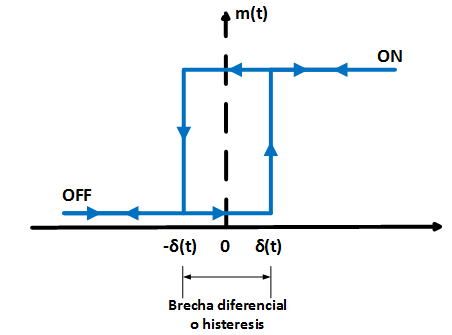
\includegraphics[width=85mm,height=50mm]{imagenes/capitulo2/2_1_On-Off}
\caption {Esquema de funcionamiento del controlador \textit{On-Off} }
\label{fig2_1:histeresis}
\end{figure}

	En dicha figura puede verse que la conmutación no se realiza en 0 sino en los extremos de un intervalo denominado \textit{brecha diferencial o histéresis}. Este mecanismo permite evitar daños en los componentes de la planta cuando la conmutación entre los 2 estados se realiza de manera muy rápida. La señal de control no conmuta hasta que la señal de error supera una cierta cantidad $\delta(t)$, tanto si el error es positivo ($e(t) > \delta(t)$) como si es negativo ($e(t) < -\delta(t)$). En ocasiones puede fijarse ese intervalo a 0, siempre y cuando la conmutación no sea muy rápida y se garantice el correcto funcionamento de la planta.

	El funcionamiento del controlador es el siguiente: supongamos que la señal de control está en OFF y el error es negativo. Cuando $e(t) > \delta(t)$, la señal de control conmuta al estado ON. Este estado habitualmente se traduce en una acción que hace que la planta a controlar se encienda y funcione (enceder un motor, abrir una válvula...). 

	Supongamos ahora que la señal de control está en ON y el error es positivo. Si se cumple que $e(t) < -\delta(t)$, la señal de control conmuta al estado OFF. Este estado habitualmente se traduce en una acción que hace que la planta a controlar se apague o deja de funcionar (apagar un motor, cerrar una válvula...).

\begin{figure}[htbp]
\centering
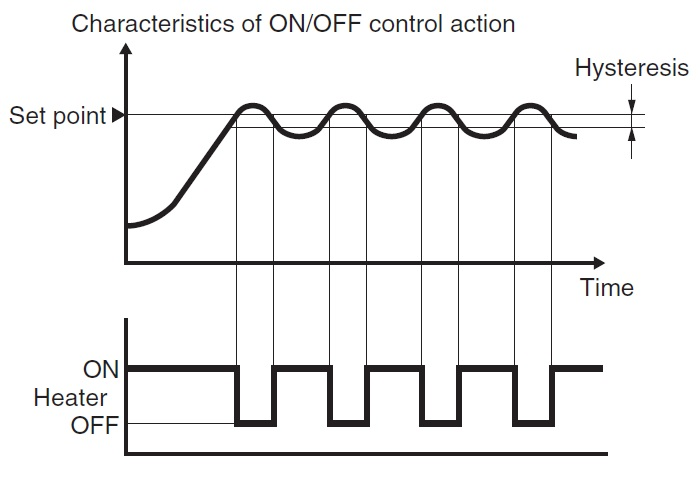
\includegraphics[width=85mm,height=45mm]{imagenes/capitulo2/2_2_On-Off}
\caption {Respuesta de un sistema con un controlador \textit{On-Off}. Fuente: Omron \cite{fabricante1}}
\label{fig2_2:on-off}
\end{figure}

	El funcionamiento del controlador es sencillo aunque presenta limitaciones en cuanto a que sólo puede usarse para aquellos sistemas que puedan ser controlados mediante 2 estados de funcionamiento.

\subsection{Controlador proporcional (P)}

	Su acción se basa en multiplicar la señal de error por una constante denominada \textit{constante proporcional} $K_{p}$. Su expresión matemática es la siguiente:
\begin{equation}\label{ecuacion2_1}
\normalsize m_{P}(t) =K_{p}e(t)
\end{equation}

	El controlador amplifica la señal de error para conseguir que la señal medida siga a la señal de referencia. Sin embargo, analizando la ecuación, se ve que no se consigue eliminar el error estacionario ya que si el error fuese nulo, la señal de control también lo sería. 

	Este controlador puede ajustarse a través de la constante $K_{p}$ o mediante el concepto de la \textbf{banda proporcional}, que se define como la cantidad que tiene que cambiar la variable controlada para lograr un cambio del 100\% en la acción de control. Su expresión matemática es  $BP\%=\frac{100}{K_{p}}$ y es un concepto similar a la ganancia proporcional. En la figura \ref{fig2_3_1:proporcional} se muestra una gráfica que representa el comportamiento de esta acción.

\begin{figure}[htbp]
\centering
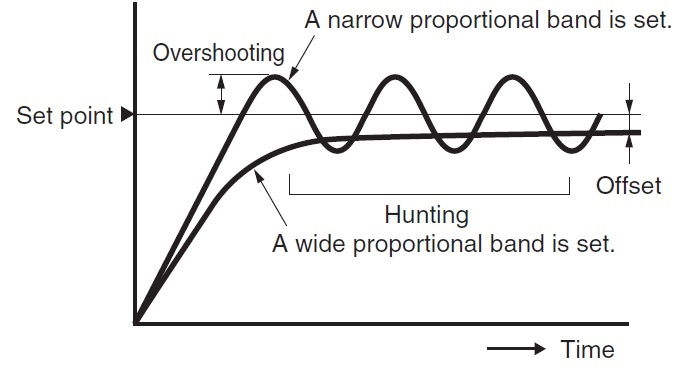
\includegraphics[width=90mm,height=45mm]{imagenes/capitulo2/2_3_1_Proporcional}
\caption {Respuesta de un sistema con un controlador P. Fuente: Omron \cite{fabricante1}}
\label{fig2_3_1:proporcional}
\end{figure}

	En dicha gráfica puede verse que si la banda proporcional es amplia (equivale a una $K_{p}$ pequeña), la respuesta de la planta se aproxima al valor de referencia pero tiene un ligero offset, mientras que si la banda es reducida (equivale a una $K_{p}$ grande), la respuesta presenta oscilaciones entorno al valor de referencia.

\subsection{Controlador Integral (I)}

	Su acción se basa en integrar la señal de error y multiplicarla por una constante denominada \textit{constante integral} $K_{i}$. Su expresión matemática es la siguiente:
\begin{equation}\label{ecuacion2_2}
\normalsize m_{I}(t) = K_{i}\int _0^t e(t) dt
\end{equation}
	
	El controlador genera una señal que es función de la "historia"~ de la señal de error, lo que permite conseguir una señal de control no nula aunque la señal de error sí lo sea. Este controlador consigue eliminar el error estacionario aunque empeora la estabilidad del sistema, aumentando el sobreimpulso de la respuesta transitoria e incluso puede hacer que el sistema se vuelva inestable.  No suele utilizarse sólo sino que se combina con otras acciones de control, por ejemplo, con un controlador proporcional.

\subsection{Controlador Proporcional Integral (PI)}

	Este controlador se basa en una combinación de la acción proporcional y la acción integral. Su expresión matemática es la siguiente:
\begin{equation}\label{ecuacion2_3}
\normalsize m_{PI}(t) =K_{p}e(t) + K_{i}\int _0^t e(t) dt = K_{p}\left( e(t) + \frac{1}{T_{i}} \int _0^t e(t) dt\right)
\end{equation}

	Ajustando los parámetros $K_{p}$ y $K_{i}$ se consigue ajustar la respuesta a los requisitos deseados. El ajuste de la acción integral puede realizarse mediante $K_{i}$  o usando un parámetro denominado \textit{tiempo integral} $T_{i}$, que se define como $T_{i}=\frac{K_{p}}{K_{i}}$.

	En la figura \ref{fig2_3_2:PI} se muestra la respuesta de una planta con este controlador. En dicha figura se observa como la acción integral consigue eliminar el error estacionario y que la respuesta se aproxime al valor deseado. Es necesario ajustar correctamente los valores $K_{p}$ y $K_{i}$, ya que puede ocurrir que la señal tenga un mayor sobreimpulso o que sea demasiado lenta y tarde más tiempo en alcanzar el estado estacionario.

\begin{figure}[htbp]
\centering
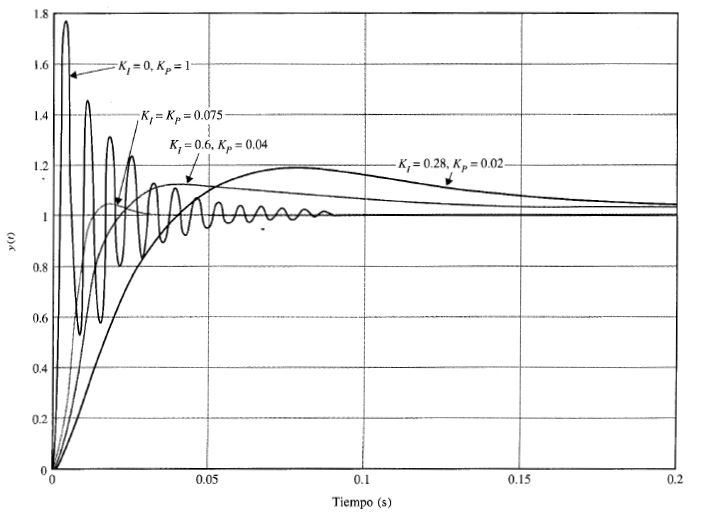
\includegraphics[width=100mm,height=55mm]{imagenes/capitulo2/2_3_2_PI}
\caption {Respuesta de un sistema con una acción PI. Fuente: \textit{Benjamin C. Kuo} \cite{control2}}
\label{fig2_3_2:PI}
\end{figure}

\subsection{Controlador Derivativavo (D)}

	Su acción se basa en derivar la señal de error y multiplicarla por una constante denominada \textit{constante derivativa} $K_{d}$. Su expresión matemática es la siguiente:
\begin{equation}\label{ecuacion2_4}
\normalsize m_{D}(t) = K_{d}\frac{de(t)}{dt}
\end{equation}

	Esta acción añade sensibilidad al sistema y permite corregir el error antes de que se vuelva excesivo. Provoca un aumento en la estabilidad relativa que se traduce en un menor sobreimpulso y una respuesta con un menor tiempo de subida y de establecimiento. Sin embargo, no puede utilizarse sólo porque no es capaz de eliminar el error estacionario para una señal constante.  Suele combinarse con otras acciones de control, por ejemplo, con un controlador proporcional.

\subsection{Controlador Proporcional Derivativo (PD)}

	Este controlador se basa en la combinación de la acción proporcional y la acción derivativa. Su expresión matemática es la siguiente:
\begin{equation}\label{ecuacion2_5}
\normalsize m_{PD}(t) =K_{p}e(t) + K_{d}\frac{de(t)}{dt} = K_{p}\left( e(t) + T_{d}\frac{de(t)}{dt}\right)
\end{equation}

	Ajustando los parámetros $K_{p}$ y $K_{d}$ se consigue ajustar la respuesta a los requisitos deseados. El ajuste de la acción derivativa puede hacerse mediante $K_{d}$ o con un parámetro denominado \textit{tiempo derivativo} $T_{d}$, que se define como $T_{d}=\frac{K_{d}}{K_{p}}$.

\begin{figure}[htbp]
\centering
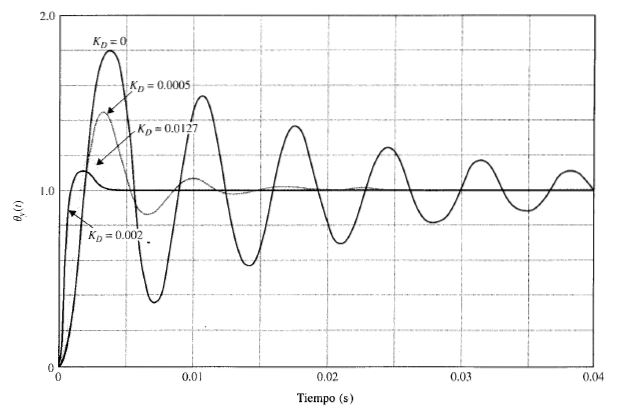
\includegraphics[width=100mm,height=55mm]{imagenes/capitulo2/2_3_3_PD}
\caption {Respuesta de un sistema con una acción PD. Fuente: \textit{Benjamin C. Kuo}\cite{control2}}
\label{fig2_3_3:PD}
\end{figure}
	
	En la figura \ref{fig2_3_3:PD} se muestra la respuesta de una planta con este controlador. En dicha figura se observa que a medida que aumenta la acción derivativa, la respuesta tiene un menor sobreimpulso, es más rápida y tiene un menor tiempo de establecimiento. 

\subsection{Controlador PID}
	Combina las ventajas de las 3 acciones . Su expresión matemática es:
\begin{equation}\label{ecuacion2_6}
\normalsize m(t) =K_{p}e(t) + K_{i}\int _0^t e(t) dt + K_{d}\frac{de(t)}{dt} =  K_{p}\left( e(t) + \frac{1}{T_{i}} \int _0^t e(t) dt + T_{d}\frac{de(t)}{dt}\right)
\end{equation}

	En la figura \ref{fig2_4:PID} se compara la respuesta de una planta usando un controlador PID frente a un controlador PI y un controlador PD. Ajustando los parámetros adecuadamente, se consiguen los resultados deseados. Este controlador es ampliamente usado en la industria debido a que puede adaptarse a un amplio rango de valores de funcionamiento y a que posee un planteamiento sencillo. 

\begin{figure}[htbp]
\centering
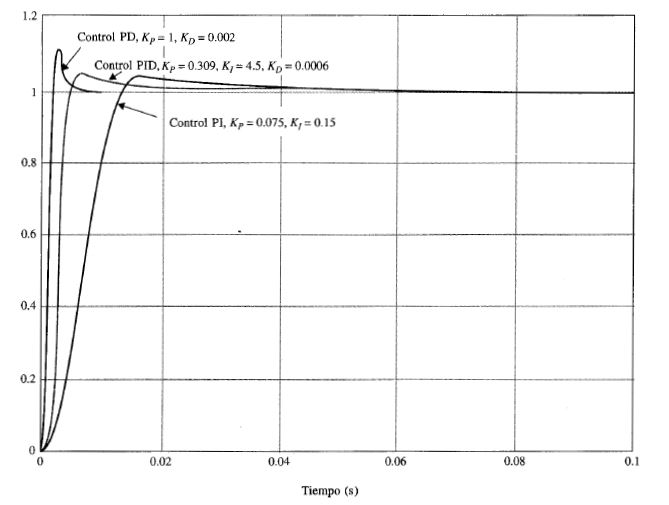
\includegraphics[width=90mm,height=55mm]{imagenes/capitulo2/2_4_PID}
\caption {Respuesta de un sistema usando un PID. Fuente: \textit{Benjamin C. Kuo} \cite{control2}}
\label{fig2_4:PID}
\end{figure}

	Este controladores posee diferentes representaciones, dependiendo de las necesidades. En la figura \ref{fig2_5:PID} se muestran algunas de ellas.  El 1º esquema es la representación paralela o ideal y se caracteriza en que cada una de las acciones no se influyen mutuamente. Su expresión matemática es la primera parte de la ecuación \ref{ecuacion2_6}.

	 El esquema central es la representación estándar o no interactiva y se basa en que la acción proporcional influye en el resto de acciones pero la acción integral y derivativa no se influyen entre sí. Su expresión matemática es la segunda parte de la ecuación \ref{ecuacion2_6}. Por último, la figura de la derecha es la representación serie o interactuante y se caracteriza porque la acción integral influye en la derivativa o vicerversa.

\begin{figure}[htbp]
\centering
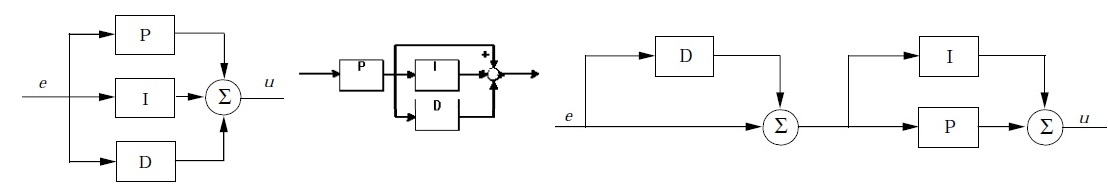
\includegraphics[width=110mm,height=30mm]{imagenes/capitulo2/2_5_PID}
\caption {Esquemas de representación de un PID. Fuente: \textit{Katsuhiko Ogata} \cite{control3}}
\label{fig2_5:PID}
\end{figure}

	Este controlador tiene un funcionamiento lineal pero en muchas ocasiones pueden aparecer efectos no lineales. Una no linealidad típica es el efecto windup. El actuador posee un rango de funcionamiento limitado y si el sistema de control tiene un amplio rango de operación, puede ocurrir que la señal de control alcance el límite del actuador.

	Cuando esto sucede, el lazo de realimentación se rompe porque el actuador se satura y deja de seguir a la señal de control. Sin embargo, el error se sigue acumulando y la señal de control sigue aumentando. Cuando la señal de error cambia de signo, la señal de control empieza a reducirse pero requiere de un gran tiempo para volver a entrar en la región lineal. Esto provoca grandes transitorios en la respuesta de la planta. En la figura \ref{fig2_6:windup} se representa este efecto.  

\begin{figure}[htbp]
\centering
\includegraphics[width=110mm,height=25mm]{imagenes/capitulo2/2_6_Windup}
\caption {Representación del efecto windup. Fuente: \textit{Katsuhiko Ogata} \cite{control3}}
\label{fig2_6:windup}
\end{figure}

	Para solucionarlo, existen varios métodos como limitar el valor de referencia para que la señal de control no alcance los límites del actuador, la integración condicional que se basa en habilitar la acción integral si se cumplen determinadas condiciones o la técnica del recálculo y seguimiento que recalcula la integral cuando el actuador se satura y consigue que la señal de control se aproxime al límite del actuador \cite{control3}. 

\section{Control de temperatura}

	En este apartado se pretende exponer cómo se realiza el control de la temperatura en un centro de datos, es decir, como se ajusta el valor de referencia según la situación del CPD.

	En la actualidad, existen diferentes herramientas de control y gestión de los centros de datos, como Data Center Infraestructure Management (DCIM) o Supervisory Control And Data Adquisition (SCADA). 

	El sistema SCADA supervisa y controla las operaciones a través de sensores que están colocados en diferentes lugares y que son monitorizados desde una unidad centralizada. Las funciones incluyen gestión de alarmas, diagnóstico, mantenimiento, interfaces gráficas que muestran la situación actual del CPD, entre otros. 

	El sistema DCIM está formado por un sistema software, hardware y sensores que permiten gestionar, supervisar y planificar la capacidad de la infraestructura crítica de un CPD. El sistema maneja los datos proporcionados por los sensores y con ellos puede gestionar tanto los servidores como el resto de equipos. Dispone de una plataforma de gestión y monitorización para visualizar el estado del CPD en tiempo real.

	Sin embargo, estos sistemas son complejos de manejar y requieren de algún tipo de intervención humana, incluyendo el caso de  la temperatura. Estos sistemas monitorizan y controlan la temperatura pero se necesita un operario para realizar los cambios.

	Por tanto, el sistema de actuación diseñado en este trabajo debe ser capaz de proporcionar al controlador el dato óptimo de temperatura de una forma automática y sin ningún tipo de acción humana.
